\documentclass[12pt]{article}
\usepackage[a4paper, total={7in, 9in}]{geometry}
\usepackage{amsmath, amssymb}
\usepackage{graphicx}
\usepackage{enumitem}
\usepackage{fancyvrb}
\usepackage[skip=\medskipamount]{parskip}
\usepackage{pdfpages}
\usepackage{array}
\usepackage{tabularray}
\usepackage{longtable}
\usepackage{tikz}
\setlength{\parindent}{0pt}

\renewcommand*{\thesubsection}{\alph{subsection}}
\renewcommand*{\theenumi}{\alph{enumi}}

\title{\vspace{-1.5cm}UMC-203 Assignment-1}
\author{Aditya Gupta \\
SR No: 22205}
\date{}

\begin{document}
\maketitle

\section*{Question 1}
\begin{enumerate}[leftmargin=*]
    \item Since the coordinates for each vector are independent, their covariance is 0. This means that the matrices $\Sigma_0$ and $\Sigma_1$ are diagonal.
    
    \medskip
    \item Let our classifier be $h(x)$. Since the Bayes classifier minimises the loss, we have:
    \begin{align*}
        h(x) = 1 &\implies l(1,0) \cdot P(X=x \ | \ Y=1) \cdot P(Y=1) < l(0,1) \cdot P(X=x \ | \ Y=0) \cdot P(Y=0) \\
        h(x) = 0 &\implies l(0,1) \cdot P(X=x \ | \ Y=0) \cdot P(Y=0) < l(1,0) \cdot P(X=x \ | \ Y=1) \cdot P(Y=1)
    \end{align*}
    We can simplify these inequalities to:
    \begin{align*}
        \frac{l(0,1)}{l(1,0)} \cdot \frac{P(X=x \ | \ Y=0)}{P(X=x \ | \ Y=1)} \cdot \frac{P(Y=0)}{P(Y=1)} > 1
    \end{align*}
    Taking log on both sides, we define:
    \begin{align*}
        f(x) = log(\frac{l(0,1)}{l(1,0)}) + log(\frac{P(X=x \ | \ Y=0)}{P(X=x \ | \ Y=1)}) + log(\frac{P(Y=0)}{P(Y=1)})
    \end{align*}
    Now $P(Y=0) = P(Y=1) = 0.5$, so the last term is 0. The class conditional probabilities are given by:
    \begin{align*}
        P(X=x \ | \ Y=0) &= \frac{1}{(2\pi)^{d/2}|\Sigma_0|^{1/2}} \cdot exp(-\frac{1}{2}(x-\mu_0)^T\Sigma_0^{-1}(x-\mu_0)) \\
        P(X=x \ | \ Y=1) &= \frac{1}{(2\pi)^{d/2}|\Sigma_1|^{1/2}} \cdot exp(-\frac{1}{2}(x-\mu_1)^T\Sigma_1^{-1}(x-\mu_1))
    \end{align*}
    Substituting these into the inequality, we get:
    \begin{align*}
        f(x) &= log(\frac{l(0,1)}{l(1,0)}) + log(\frac{|\Sigma_1|}{|\Sigma_0|}) + \frac{1}{2}((x-\mu_0)^T\Sigma_0^{-1}(x-\mu_0) - (x-\mu_1)^T\Sigma_1^{-1}(x-\mu_1)) \\
        &= log(\frac{l(0,1)}{l(1,0)}) + log(\frac{|\Sigma_1|}{|\Sigma_0|}) + \frac{1}{2}x^T(\Sigma_0^{-1}-\Sigma_1^{-1})x - (\mu_0^T\Sigma_0^{-1}-\mu_1^T\Sigma_1^{-1})x + \frac{1}{2}(\mu_0^T\Sigma_0^{-1}\mu_0 - \mu_1^T\Sigma_1^{-1}\mu_1)
    \end{align*}
    Thus the classifier is:
    \begin{align*}
        h(x) = \begin{cases}
            1 & \text{if } f(x) > 0 \\
            0 & \text{otherwise}
        \end{cases}
    \end{align*}

    \medskip
    \item n = 2
    \begin{align*}
        \mu_0 &= \begin{pmatrix}
            -1.96221, & 0.18944, & -0.049585, & 0.081975, & 1.9774
        \end{pmatrix}^T \\
        \mu_1 &= \begin{pmatrix}
            1.20234, & 2.34644, & 0.714605, & 0.214555, & -0.690705 \\
        \end{pmatrix}^T \\ \\
        \Sigma_0 &= \begin{pmatrix}
            0.30358998 & 0 & 0 & 0 & 0 \\
            0 & 0.11507021 & 0 & 0 & 0 \\
            0 & 0 & 0.3862809 & 0 & 0 \\
            0 & 0 & 0 & 0.00121766 & 0 \\
            0 & 0 & 0 & 0 & 0.27284952 
        \end{pmatrix} \\ \\
        \Sigma_1 &= \begin{pmatrix}
            0.36590401 & 0 & 0 & 0 & 0 \\
            0 & 2.27448626 & 0 & 0 & 0 \\
            0 & 0 & 3.57434945 & 0 & 0 \\
            0 & 0 & 0 & 0.60563415 & 0 \\
            0 & 0 & 0 & 0 & 0.18616205
        \end{pmatrix}
    \end{align*}

    \vspace*{1cm}
    n = 10
    \begin{align*}
        \mu_0 &= \begin{pmatrix}
            -1.224015, & -0.489617, & -1.660371, & -1.284154, & -0.8959
        \end{pmatrix}^T \\
        \mu_1 &= \begin{pmatrix}
            0.866145, & 1.660201, & 1.566222, & 1.151618, & 1.596393 \\
        \end{pmatrix}^T \\ \\
        \Sigma_0 &= \begin{pmatrix}
            2.57804484 & 0 & 0 & 0 & 0 \\
            0 & 2.79660319 & 0 & 0 & 0 \\
            0 & 0 & 1.29792628 & 0 & 0 \\
            0 & 0 & 0 & 0.51546087 & 0 \\
            0 & 0 & 0 & 0 & 3.16155971 
        \end{pmatrix} \\ \\
        \Sigma_1 &= \begin{pmatrix}
            1.53072143 & 0 & 0 & 0 & 0 \\
            0 & 2.1998811 & 0 & 0 & 0 \\
            0 & 0 & 1.96567014 & 0 & 0 \\
            0 & 0 & 0 & 1.06477637 & 0 \\
            0 & 0 & 0 & 0 & 4.03515874
        \end{pmatrix}
    \end{align*}

    n = 20
    \begin{align*}
        \mu_0 &= \begin{pmatrix}
            -1.5337625, & -0.97972, & -0.855086, & -0.648637, & -0.4467095
        \end{pmatrix}^T \\
        \mu_1 &= \begin{pmatrix}
            0.821065, & 1.585292, & 0.9529255, & 0.933732, & 1.3502465 \\
        \end{pmatrix}^T \\ \\
        \Sigma_0 &= \begin{pmatrix}
            2.48649536 & 0 & 0 & 0 & 0 \\
            0 & 2.36520239 & 0 & 0 & 0 \\
            0 & 0 & 2.38199098 & 0 & 0 \\
            0 & 0 & 0 & 0.88413231 & 0 \\
            0 & 0 & 0 & 0 & 8.81874419 
        \end{pmatrix} \\ \\
        \Sigma_1 &= \begin{pmatrix}
            2.05641534 & 0 & 0 & 0 & 0 \\
            0 & 2.5038535 & 0 & 0 & 0 \\
            0 & 0 & 2.00793081 & 0 & 0 \\
            0 & 0 & 0 & 0.83759293 & 0 \\
            0 & 0 & 0 & 0 & 3.65894733
        \end{pmatrix}
    \end{align*}

    \vspace*{1cm}
    n = 50
    \begin{align*}
        \mu_0 &= \begin{pmatrix}
            -0.6546238, & -0.9917164, & -0.6672196, & -1.2205246, & -1.2043944
        \end{pmatrix}^T \\
        \mu_1 &= \begin{pmatrix}
            0.787225, & 1.1853278, & 0.936112, & 1.0084708, & 1.5183972 \\
        \end{pmatrix}^T \\ \\
        \Sigma_0 &= \begin{pmatrix}
            1.99685417 & 0 & 0 & 0 & 0 \\
            0 & 2.52477144 & 0 & 0 & 0 \\
            0 & 0 & 2.24238608 & 0 & 0 \\
            0 & 0 & 0 & 1.2040245 & 0 \\
            0 & 0 & 0 & 0 & 4.87413308 
        \end{pmatrix} \\ \\
        \Sigma_1 &= \begin{pmatrix}
            2.25806098 & 0 & 0 & 0 & 0 \\
            0 & 2.25062163 & 0 & 0 & 0 \\
            0 & 0 & 2.19810184 & 0 & 0 \\
            0 & 0 & 0 & 0.94272801 & 0 \\
            0 & 0 & 0 & 0 & 6.42619665
        \end{pmatrix}
    \end{align*}

    n = 100
    \begin{align*}
        \mu_0 &= \begin{pmatrix}
            -0.9689749, & -0.9270526, & -0.9664571, & -0.8201764, & -1.0597007
        \end{pmatrix}^T \\
        \mu_1 &= \begin{pmatrix}
            1.0663006, & 1.0968057, & 1.1344462, & 0.8939731, & 1.1570014 \\
        \end{pmatrix}^T \\ \\
        \Sigma_0 &= \begin{pmatrix}
            2.28345333 & 0 & 0 & 0 & 0 \\
            0 & 2.40552193 & 0 & 0 & 0 \\
            0 & 0 & 2.21243518 & 0 & 0 \\
            0 & 0 & 0 & 0.8616304 & 0 \\
            0 & 0 & 0 & 0 & 5.95635315 
        \end{pmatrix} \\ \\
        \Sigma_1 &= \begin{pmatrix}
            2.20534076 & 0 & 0 & 0 & 0 \\
            0 & 2.3955327 & 0 & 0 & 0 \\
            0 & 0 & 2.25958041 & 0 & 0 \\
            0 & 0 & 0 & 1.08648598 & 0 \\
            0 & 0 & 0 & 0 & 5.78077179
        \end{pmatrix}
    \end{align*}

    \vspace*{1cm}
    n = 500
    \begin{align*}
        \mu_0 &= \begin{pmatrix}
            -1.01377356, & -0.99894404, & -1.0104815, & -1.00787736, & -0.93998246
        \end{pmatrix}^T \\
        \mu_1 &= \begin{pmatrix}
            1.01445284, & 1.01366632, & 0.97896886, & 1.04943584, & 1.0113819 \\
        \end{pmatrix}^T \\ \\
        \Sigma_0 &= \begin{pmatrix}
            2.35045986 & 0 & 0 & 0 & 0 \\
            0 & 2.46591919 & 0 & 0 & 0 \\
            0 & 0 & 2.37234442 & 0 & 0 \\
            0 & 0 & 0 & 0.94806002 & 0 \\
            0 & 0 & 0 & 0 & 5.37868451 
        \end{pmatrix} \\ \\
        \Sigma_1 &= \begin{pmatrix}
            2.37126345 & 0 & 0 & 0 & 0 \\
            0 & 2.50692838 & 0 & 0 & 0 \\
            0 & 0 & 2.29197777 & 0 & 0 \\
            0 & 0 & 0 & 0.95968702 & 0 \\
            0 & 0 & 0 & 0 & 5.2598086
        \end{pmatrix}
    \end{align*}

    n = 1000
    \begin{align*}
        \mu_0 &= \begin{pmatrix}
            -1.05463798, & -1.03853627, & -1.01758959, & -1.03431583, & -0.90236216
        \end{pmatrix}^T \\
        \mu_1 &= \begin{pmatrix}
            1.00033964, & 1.00736114, & 0.98424368, & 1.02077924, & 1.03569972 \\
        \end{pmatrix}^T \\ \\
        \Sigma_0 &= \begin{pmatrix}
            2.29483634 & 0 & 0 & 0 & 0 \\
            0 & 2.50030068 & 0 & 0 & 0 \\
            0 & 0 & 2.41024345 & 0 & 0 \\
            0 & 0 & 0 & 1.08015965 & 0 \\
            0 & 0 & 0 & 0 & 5.41893795 
        \end{pmatrix} \\ \\
        \Sigma_1 &= \begin{pmatrix}
            2.36106084 & 0 & 0 & 0 & 0 \\
            0 & 2.48646354 & 0 & 0 & 0 \\
            0 & 0 & 2.33218892 & 0 & 0 \\
            0 & 0 & 0 & 0.95469472 & 0 \\
            0 & 0 & 0 & 0 & 5.31983791
        \end{pmatrix}
    \end{align*}

    \vspace*{1cm}
    \item The misclassification loss is calculated by dividing the net loss by the number of samples. The net loss is calculated by summing the loss for each sample. The losses given were:
    \begin{align*}
        l(0,1) &= 5 \\
        l(1,0) &= 3
    \end{align*}
    For the above data, the misclassification loss is as follows:

    \begin{center}
        \begin{tabular}{|c|c|}
            \hline
            n & Misclassification Loss \\
            \hline
            2 & 1.475 \\
            10 & 0.265 \\
            20 & 0.4 \\
            50 & 0.25 \\
            100 & 0.34 \\
            500 & 0.24 \\
            1000 & 0.265 \\
            \hline
        \end{tabular}
    \end{center}

    \vspace*{1cm}
    \item For the CIFAR10 dataset, we use the same classifier as before. Out of the 4000 sample images, we get 2000 misclassification errors. Thus the accuracy is 50\%.
\end{enumerate}

\pagebreak
\section*{Question 2}
\begin{enumerate}
    \item w = [13.44741, 14.15805, 13.29934, 40.93782,  7.18301], b = 0.0
    \item Number of errors = 780
    \item Margin = 0.0009899721747263753
    \item Radius of data set = 4.582303697355731
    \item w reported in the file AIML\_2024\_A1\_22205\_q2\_w.csv, b = -2.0
    \item Number of errors = 216
    \item Margin = 2.0970062891016434
    \item Radius of data set = 3881.4121141666983
\end{enumerate}


\section*{Question 3}
\subsection*{IRIS Dataset}
\begin{enumerate}[leftmargin=*]
    \item The projection vector is given by:
    \begin{align*}
        w = \frac{(\Sigma_0 + \Sigma_1)^{-1}(\mu_1 - \mu_0)}{||(\Sigma_0 + \Sigma_1)^{-1}(\mu_1 - \mu_0)||}
    \end{align*}
    Here we have:
    \begin{align*}
        \mu_0 &= \begin{pmatrix}
            5.006, & 3.428, & 1.462, & 0.246
        \end{pmatrix}^T \\
        \mu_1 &= \begin{pmatrix}
            6.588, & 2.974, & 5.552, & 2.026
        \end{pmatrix}^T \\ \\ 
        \Sigma_0 &= \begin{pmatrix}
            0.12424898 & 0.09921633 & 0.0163551 & 0.01033061 \\
            0.09921633 & 0.1436898 & 0.01169796 & 0.00929796 \\
            0.0163551 & 0.01169796 & 0.03015918 & 0.00606939 \\
            0.01033061 & 0.00929796 & 0.00606939 & 0.01110612
        \end{pmatrix} \\ \\
        \Sigma_1 &= \begin{pmatrix}
            0.40434286 & 0.09376327 & 0.3032898 & 0.04909388 \\
            0.09376327 & 0.10400408 & 0.07137959 & 0.04762857 \\
            0.3032898 & 0.07137959 & 0.30458776 & 0.04882449 \\
            0.04909388 & 0.04762857 & 0.04882449 & 0.07543265 
        \end{pmatrix}
    \end{align*}
    From this, we get:
    \begin{align*}
        w &= \begin{pmatrix}
            -0.28543316, & -0.2165812, & 0.65799713, & 0.66231433
        \end{pmatrix}^T
    \end{align*}
    We set the value of b as:
    \begin{align*}
        b &= -w^T(\frac{\mu_0 + \mu_1}{2}) \\
        &= -0.7120525349911115
    \end{align*}

    \item The histogram for the projection of the data onto the vector w:
    \begin{center}
        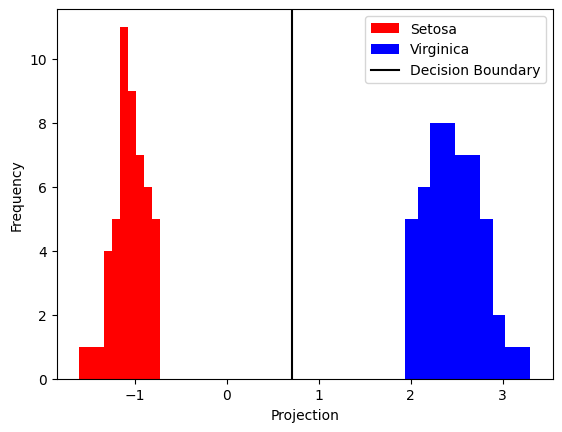
\includegraphics{img/iris.png}
    \end{center}
\end{enumerate}

\subsection*{Oracle Dataset}
\begin{enumerate}
    \item The projection vector is given by:
    \begin{align*}
        w = \frac{(\Sigma_0 + \Sigma_1)^{-1}(\mu_1 - \mu_0)}{||(\Sigma_0 + \Sigma_1)^{-1}(\mu_1 - \mu_0)||}
    \end{align*}
    Here we have:
    \begin{align*}
        \mu_0 &= \begin{pmatrix}
            4.99600361e-17, & 2.63677968e-17
        \end{pmatrix}^T \\
        \mu_1 &= \begin{pmatrix}
            1.49880108e-17, & -5.55111512e-18
        \end{pmatrix}^T \\ \\ 
        \Sigma_0 &= \begin{pmatrix}
            5.05050505e-01 & 4.49180132e-18 \\
            4.49180132e-18 & 5.05050505e-01
        \end{pmatrix} \\ \\
        \Sigma_1 &= \begin{pmatrix}
            6.90211637e-02 & 2.61041869e-18 \\
            2.61041869e-18 & 6.90211637e-02
        \end{pmatrix}
    \end{align*}
    From this, we get:
    \begin{align*}
        w &= \begin{pmatrix}
            -0.73861239 & -0.67413036
        \end{pmatrix}^T
    \end{align*}

    \bigskip
    The histogram for the projection of the data onto the vector w:
    \begin{center}
        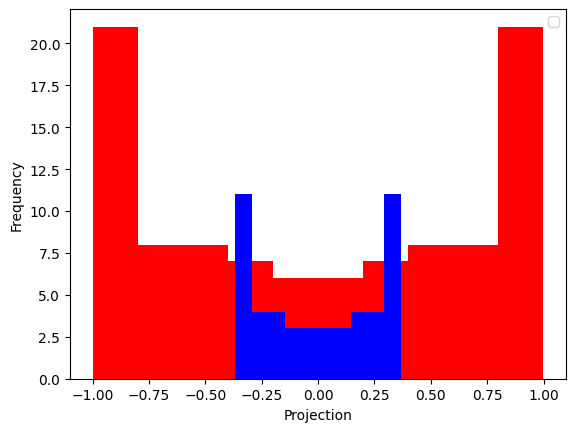
\includegraphics{img/oracle.png}
    \end{center}
    This projected data is not linearly separable.

    \vspace*{0.5cm}
    \item The projection vector is given by:
    \begin{align*}
        w = \frac{(\Sigma_0 + \Sigma_1)^{-1}(\mu_1 - \mu_0)}{||(\Sigma_0 + \Sigma_1)^{-1}(\mu_1 - \mu_0)||}
    \end{align*}
    Here we have:
    \begin{align*}
        \mu_0 &= \begin{pmatrix}
            4.99600361e-17, & 2.63677968e-17, & 5.00000000e-01, & 5.00000000e-01
        \end{pmatrix}^T \\
        \mu_1 &= \begin{pmatrix}
            1.49880108e-17, & -5.55111512e-18, & 6.76407405e-02, & 6.76407405e-02
        \end{pmatrix}^T \\ \\ 
        \Sigma_0 &= \begin{pmatrix}
            5.05050505e-01 & 4.49180132e-18 & 4.42012213e-17 & -3.85940343e-17 \\
            4.49180132e-18 & 5.05050505e-01 & -1.14183654e-17 & 5.25045973e-18 \\
            4.42012213e-17 & -1.14183654e-17 & 1.26262626e-01 & -1.26262626e-01 \\
            -3.85940343e-17 & 5.25045973e-18 & -1.26262626e-01 & 1.26262626e-01
        \end{pmatrix} \\ \\
        \Sigma_1 &= \begin{pmatrix}
            6.90211637e-02 & 2.61041869e-18 & 2.54151354e-18 & -2.61981252e-18 \\
            2.61041869e-18 & 6.90211637e-02 & 3.88525119e-19 & -9.63539806e-19 \\
            2.54151354e-18 & 3.88525119e-19 & 2.33432131e-03 & -2.33432131e-03 \\
            -2.61981252e-18 & -9.63539806e-19 & -2.33432131e-03 & 2.33432131e-03
        \end{pmatrix}
    \end{align*}
    To get w, we need to add a small offset to the covariance matrices since their sum is becoming a singular matrix, which is not invertible. From this, we get:
    \begin{align*}
        w &\approx \begin{pmatrix}
            0, & 0, & -0.70711, & -0.70711
        \end{pmatrix}^T
    \end{align*}
    We set the value of b as:
    \begin{align*}
        b &= -w^T(\frac{\mu_0 + \mu_1}{2}) \\
        &= 0.40138444398314743
    \end{align*}
    This projected data is linearly separable.

    \bigskip
    \item The histogram for the projection of the transformed data onto the vector w:
    \begin{center}
        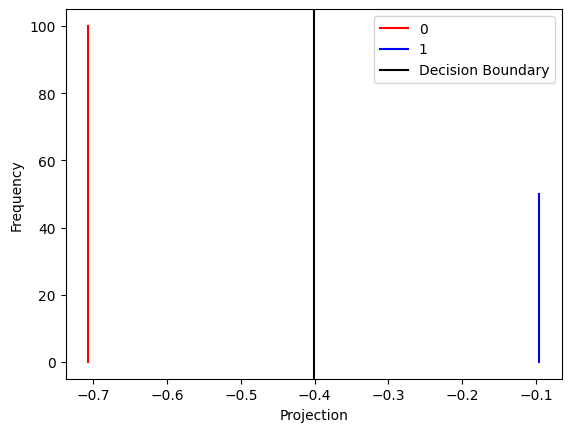
\includegraphics{img/transform.png}
    \end{center}

    \item The accuracy for different threshold values is:
    \begin{center}
        \begin{tabular}{|c|c|}
            \hline
            Threshold & Accuracy \\
            \hline
            0.1 & 70\% \\
            0.2 & 87\% \\
            0.3 & 94\% \\
            0.4 & 93\% \\
            0.5 & 93\% \\
            0.6 & 85\% \\
            0.7 & 80\% \\
            \hline
        \end{tabular}
    \end{center}
\end{enumerate}


\section*{Question 4}
\begin{enumerate}[leftmargin=*]
    \item On performing the 6-fold cross validation, we get the following accuracies:
    \begin{align*}
        \text{Cross Validation Score} &= \begin{pmatrix} 0.74, 0.81, 0.72, 0.77, 0.75, 0.88 \end{pmatrix} \\
        \text{Mean Cross Validation Score} &= 0.778333
    \end{align*}

    \item The confusion matrix for the test data is:
    \[
    \begin{pmatrix}
        \begin{bmatrix}
            54 & 9 \\
            17 & 21 
        \end{bmatrix},
        \begin{bmatrix}
            59 & 3 \\
            16 & 22 
        \end{bmatrix},
        \begin{bmatrix}
            48 & 13 \\
            15 & 24 
        \end{bmatrix},
        \begin{bmatrix}
            57 & 5 \\
            18 & 20 
        \end{bmatrix},
        \begin{bmatrix}
            59 & 11 \\
            14 & 16 
        \end{bmatrix},
        \begin{bmatrix}
            72 & 2 \\
            10 & 16 
        \end{bmatrix}
    \end{pmatrix}
    \]

    The recall, precision, accuracy and F1-score are:
    \begin{align*}
        \text{Recall} &= \begin{pmatrix} 0.54054, 0.57894, 0.61538, 0.52631, 0.53334, 0.61538 \end{pmatrix} \\
        \text{Precision} &= \begin{pmatrix} 0.68965, 0.88, 0.64864, 0.8, 0.59259, 0.88889 \end{pmatrix} \\
        \text{Accuracy} &= \begin{pmatrix} 0.74, 0.81, 0.72, 0.77, 0.75, 0.88 \end{pmatrix} \\
        \text{F1-Score} &= \begin{pmatrix} 0.60606, 0.698412, 0.63157, 0.63492, 0.561403, 0.72727 \end{pmatrix}
    \end{align*}

    \item The bar plot of all metrics for all K models is:
    \begin{center}
        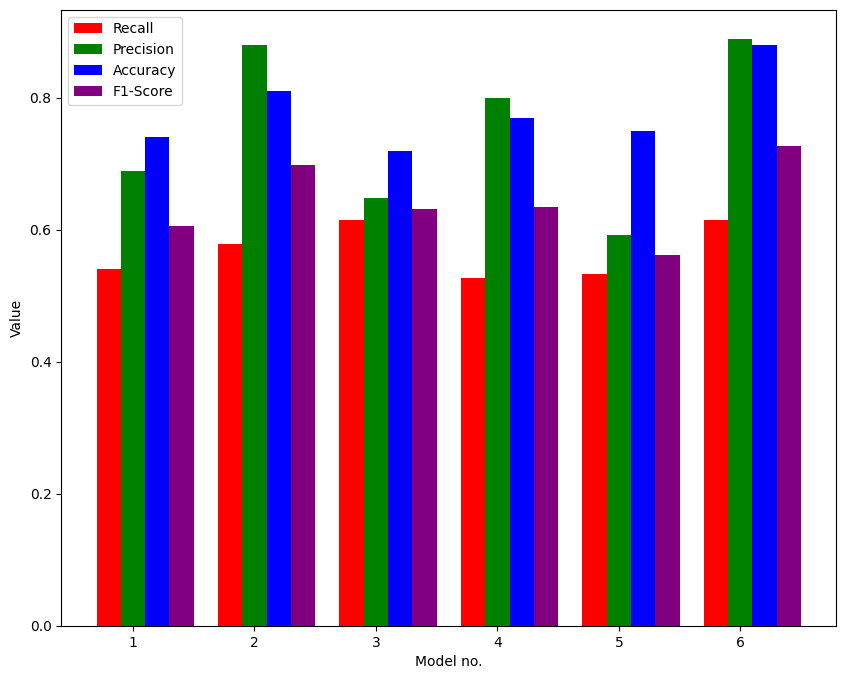
\includegraphics[height=10cm, width=12.5cm]{img/barplot.png}
    \end{center}

    \item The predictions for the test data is provided in the file AIML\_2024\_A1\_22205\_q4test.csv. The first 6 rows are the predictions from the 6 K-fold cross validation models, and the last row is the prediction from the model trained on the entire dataset.
\end{enumerate}


\end{document}
